\chapter{State of the art}
\label{chap:sota}
%====================================================%
%                     BPMN2BPEL                      %
%====================================================%
\section{BPMN to BPEL Transformation}
In the BPMN Specification, the mapping from BPMN to BPEL has been included since the first version. In fact the development of BPMN was driven by the lack of standard notation for the WS-BPEL\cite{weidlich2008}. The limitation of the mapping from BPMN to BPEL has also been discussed in various papers, focusing the issues resulting from the incompatibility of the graph structured BPMN and the block structured BPEL, and led to some more sophisticated mapping such as the one introduced by Ouyang et al. (\cite{Ouyang2006a},\cite{Ouyang2006b}).

At the moment, there are some tools that supports the transformation from BPMN to BPEL. 
In the VSDT, a mapping from BPMN to BPEL based on the mapping given in the BPMN specification was also developed \cite{TK07}, covering nearly every mapping given in the specification including event handlers, inclusive OR and event based XOR Gateways. 

For this Project the mapping from BPMN to BPEL given in the BPMN specification are used to gain a better understanding of the notation's semantics.


%====================================================%
%                     BPMN2Agents                    %
%====================================================%
%======== Existing Transformation to Jiac ===========%
\section{Existing Transformation to JiacV}
At the moment the VSDT is already equipped with a transformation of BPMN to JiacV, which generates JADL files.
As mentioned in chapter \ref{chap:background}, both JADL and Agent Bean are tools to implement the functionality of an Agent in Jiac. 
The transformation to Jiac Agent Beans is in no way a replacement to the existing transformation. Instead both transformations shall complement each other as the products of both transformations have their own advantages, some of which we can find in the following table \ref{tab:benefits}
\begin{table}[htbp]
	\centering
		\begin{tabularx}{\linewidth}{|l|X|}\hline\hline
			\multicolumn{2}{|c|}{\textbf{Advantages of:}} \\\hline
			\multicolumn{1}{|c|}{JADL} & \multicolumn{1}{c|}{Agent Beans}\\\hline
			can be deployed to a running Agent &  Written fully in Java, therefore developer friendly.\\
																				 &  Java is more powerful (expressive) that JADL.\\
			                           				 &  Better performance because no parser is involved.\\\hline\hline
		\end{tabularx}
		\caption{Advantages of JADL and Agent Beans}
		\label{tab:benefits}
\end{table}

\newpage
Because JADL files can be deployed to a running Agent, the mapping to JADL is suitable for creating dynamic behaviors and services that might be changed and deployed at runtime, while the mapping to JIAC Agent Beans (because of its expressiveness and better performance) is a better choice for creating the core components of an agent. 


\section{Workflows and Agents Development Environment}
\label{sec:wade}
A similar approach (designing agents behavior with processes and transforming it into Java Code) has been developed by the Telecom Italia with their Java Agent Development Framework (JADE) extension called Workflows and Agents Development Environment (WADE). While JADE was developed to simplify the implementation of Software Agents, WADE extended JADE with a workflow engine, making it possible to create Agents that executes tasks defined as workflows.

\subsection{Java Agent Development Framework}
JADE \cite{FBGCAPGR08, FBAPGR99} is an application framework and a middleware written in Java, which support the development of software agents. The framework  provides distributed runtime environments, agent and behavior abstractions as well as communications between agents and discovery mechanisms. We can say that its role is very similar to JIAC.

\subsection{Workflows and Agents Development Environment}
WADE \cite{WEB} is an extension to JADE, which enrich the application framework with a workflow engine. The WorkflowEngineAgent extends the JADE basic Agent class with an ability to execute workflows represented in a WADE specific formalism.

A WADE workflow is actually a Java Class, thus it can be edited and managed as Java classes and can contain pieces of code which is needed to implement the process. With WOLF, a development environment that comes with WADE, developers can edit the Workflow graphically as well as textually. The code view and the graphical view of the workflow are kept in sync.

Despite having all the advantages of a Java code, the WADE workflow is rather simple and not so expressive as the BPMN. Similarity to the agent technology such as event handling and communication flow are also missing in the workflow. Further because each workflow model is associated to a single java class, it is targeting a single agent and is not very suitable in designing multi agent systems. In the following we will take a closer look on the workflow concept of WADE. 


\subsection{Workflow Metamodel - Graphical View}
For the graphical view of the workflow, WADE adopts a workflow metamodel quite similar to that defined in the XML Process Definition Language (XPDL) standard defined by the Workflow Management Consortium (www.wfmc.org). In figure \ref{fig:wade_elements} (image taken from \cite{GCDGMB08}), we can see an example process summarizing the main elements of the WADE metamodel.
\begin{figure}[h]
	\centering
		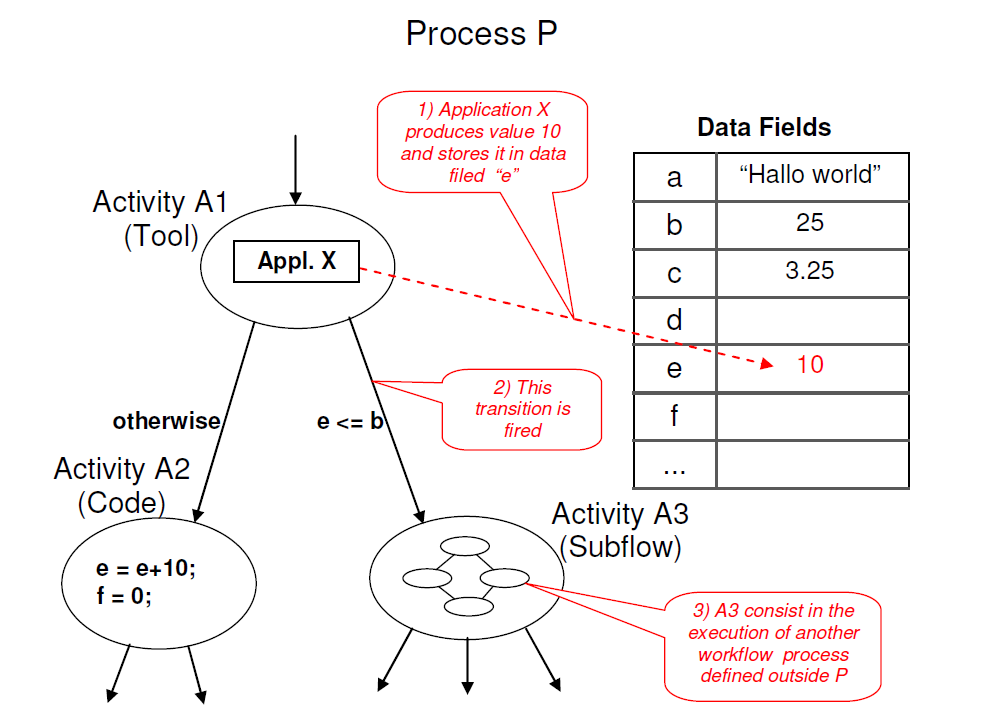
\includegraphics[width=1.00\textwidth]{images/wade_elements.png}
	\caption{Elements of WADE Metamodel \cite{GCDGMB08}}
	\label{fig:wade_elements}
\end{figure}

A Process in WADE is made up from a set of Activities, where each activity corresponds to the execution of the given operations. A Process is defined with exactly one \textbf{Start Activity}, and one or multiple \textbf{End Activities}. A Process may have Formal Parameters, which defines the type of required inputs and expected outputs.

Activities in WADE are divided into different types depending on the operations included in the activity. 6 types are mentioned in \cite{GCWADEUG10} for being the most relevant:
\begin{itemize}
	\item \textbf{\textit{Tool Activities}}\\
	      Contains the invocation of one or more \textbf{Applications}, computational entities defined outside of the workflow process and wrapped by a uniform interface.
	\item \textbf{\textit{Subflow Activities}}\\
	      Contains the invocation of another workflow process. The execution of the subflow takes place in a different computational place and it may be carried out by another agent. Further we can set whether the subflow should be executed synchronously or asynchronously.
	\item \textbf{\textit{Webservice Activities}}\\
				Contains the invocation of a webservice.
	\item \textbf{\textit{Code Activities}}\\
				Included operations are specified directly by a set of Java code. 
	\item \textbf{\textit{Subflow Join}} \\
	      Included operations consist of blocking the main workflow process and wait until the previously launched asynchronous subflow completes, and getting the results.
	\item \textbf{\textit{Route Activities}}\\
				Route activities are empty. No operations is included. It can be used to simplify complex flows. 
\end{itemize}
% explain the WADE-Workflow, add screnshots etc.
Each non ending activity has one or more outgoing \textbf{\textit{Transitions}} leading to another activity. A transition may be associated with a condition. Once an activity completes, the conditions of all outgoing transitions will be checked. If the condition holds, the transition will be fired and the workflow continues with the execution of the destination activity.

A Process has a set of \textbf{DataFields} which can be referenced anywhere in the process e.g. in the condition of a transaction or in the operations included in an activity. 
\\\\

\subsection{Workflow Implementation (Code View)}
As mentioned before, workflow in WADE is actually a (well structured) Java class. A workflow process is implemented by a Java class extending the \verb|WorkflowBehaviour| class, which provides the methods \verb|registerActivity()| and \verb|registerTransition()| for adding activities and transitions into the process. 

The \verb|registerActivity()| method takes a behavior object as argument. There are different behavior classes corresponding to the different activity types discussed in the previous subsection. The actual operations included for the registered activity are wrapped in a void method of the workflow class. The method's name is derived from the activity's name added with the ''execute'' prefix e.g \verb|executecheckBalance()| for the activity ''checkBalance''.  

The \verb|registerTransition()| method takes a Transition object as an argument. If the transition is associated with a condition, then a boolean method (with the prefix ''check'' added to the condition name) will be created.

In Figure \ref{fig:wade_graph} we can see an example process in its graphical view and Listing \ref{list:wade_code} shows the equivalent code view to the example. 

\begin{figure}[h]
		\centering
		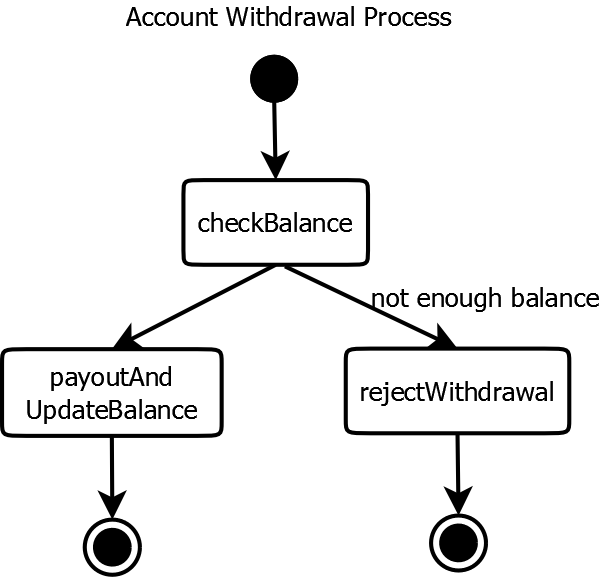
\includegraphics[width=0.5\textwidth]{images/wade_example.png}
		\caption{WADE example: Account Withdrawal Process (graphical view)}
	  \label{fig:wade_graph}
\end{figure}
\newpage
\begin{lstlisting}[language = Java, caption=WADE example: Account Withdrawal Process (code view), label = list:wade_code]
//the layout information of the graphical view
@WorkflowLayout(entryPoint = @MarkerLayout(position = "(260,31)", activityName = "checkBalance"), exitPoints = { }, transitions = {@TransitionLayout(to = "rejectWithdrawal", from = "checkBalance"), @TransitionLayout(to = "payoutAndUpdateBalance", from = "checkBalance") }, activities = {@ActivityLayout(position = "(357,175)", name = "rejectWithdrawal"), @ActivityLayout(position = "(116,171)", name = "payoutAndUpdateBalance"), @ActivityLayout(position = "(222,78)", name = "checkBalance") })

public class AccountWithdrawal extends Workflowbehavior {
	//Data fields
	public static final String NOTENOUGHBALANCE_CONDITION = "notEnoughBalance";
	public static final String REJECTWITHDRAWAL_ACTIVITY = "rejectWithdrawal";
	public static final String PAYOUTANDUPDATEBALANCE_ACTIVITY = "payoutAndUpdateBalance";
	public static final String CHECKBALANCE_ACTIVITY = "checkBalance";
	private double balance;
	
	//formal Parameter
	@FormalParameter(mode=FormalParameter.INPUT)
	public double amountToBeWithdrawn;
	
	// All activities should be registered in this method
	private void defineActivities() {
		CodeExecutionbehavior checkBalanceActivity = new CodeExecutionbehavior(
				CHECKBALANCE_ACTIVITY, this);
		registerActivity(checkBalanceActivity, INITIAL);
		CodeExecutionbehavior payoutAndUpdateBalanceActivity = new CodeExecutionbehavior(
				PAYOUTANDUPDATEBALANCE_ACTIVITY, this);
		registerActivity(payoutAndUpdateBalanceActivity, FINAL);
		CodeExecutionbehavior rejectWithdrawalActivity = new CodeExecutionbehavior(
				REJECTWITHDRAWAL_ACTIVITY, this);
		registerActivity(rejectWithdrawalActivity, FINAL);
	}

	// All transitions should be registered here
	private void defineTransitions() {
		registerTransition(new Transition(), CHECKBALANCE_ACTIVITY,
				PAYOUTANDUPDATEBALANCE_ACTIVITY);
		registerTransition(new Transition(NOTENOUGHBALANCE_CONDITION, this),
				CHECKBALANCE_ACTIVITY, REJECTWITHDRAWAL_ACTIVITY);
	}

  //activity methods
	protected void executecheckBalance() throws Exception {
		[code for checking the account's balance]
	}

	protected void executepayoutAndUpdateBalance() throws Exception {
	  [...]
	}

	protected void executerejectWithdrawal() throws Exception {
		[...]
	}

	//check method for the condition of a transition
	protected boolean checknotEnoughBalance() throws Exception {
		return true;
	}

}
\end{lstlisting}

From the above listing, we can see the structure of a workflow implementation class in WADE. At line 3, we can see how the layout information for the graphical view is coded with the Java annotation mechanism. Data fields are implemented as a class variable (line 6-10) so that it can be referenced everywhere in the workflow process. 

Although it is not strictly necessary, all activities and transitions should be registered in the methods \verb|defineActivities()| and \verb|defineTransitions()| because the graphical editor will search these methods to detect the activities and transitions to show.

In line 38 to 47 we can see the activity methods that wraps the operations included in an activity. And finally we can see the boolean method  \verb|checknotEnoughBalance()| that checks for the condition of the transition from checkBalance to rejectWithdrawal. These methods are per default empty, leaving the operations to be added directly into the code by the developer.

WADE's approach in implementing the workflow as Java code has inspired us for this project. Some of the concepts e.g wrapping the activity in a Java method can also be found in our BPMN to Agent Bean transformation. 